\documentclass[../main.tex]{subfiles}
\graphicspath{{\subfix{../images/}}}

\begin{document}
\subsection{Cooling particles using Lasers}

\tab Cooling particles is essential to most physics applications. In this case, cooling is the enemy of decoherence. Also, it can lead to trapping, which will be expanded upon in later chapters. In this chapter, we will analyze some important theories and methods to cooling subatomic particles.
\par To understand how we can use lasers to cool particles, firstly we need to expand on Wave–particle duality, particle resonance frequency and the Doppler effect.

\subsubsection{Wave–particle duality}
\tab Wave particle duality is a concept in Quantum mechanics stating that quantum entities exhibit both wave and particle properties. Important wave properties: Wavelength, Frequency. Important particle properties: mass, momentum, position. 

De Broglie equation:

\begin{equation}
    \lambda_D = \frac{\hbar}{mv}
    \label{eq: De Broglie}
\end{equation}

where $\lambda_D$ is the wave length of the particle, $\hbar$ is h-bar and m, v are the mass and velocity of the particle respectively.

From thermodynamics, we know that

\begin{equation}
    v^2 \propto T
    \label{eq: thermodynamics}
\end{equation}

where T is the temperature in absolute scale.

Combining \cref{eq: De Broglie,eq: thermodynamics}, we have:

\begin{equation}
    \lambda_D \propto \frac{1}{\sqrt{T}}
\end{equation}

In conclusion, the de Broglie wavelength of a particle is inversely proportional to its absolute Temperature. This is very important, as a lower temperature means a bigger wavelength, so the particle (molecule or ion) starts behaving as a wave even at relatively large scale (measurable in a Lab).

\subsubsection{Particle resonance frequency}
Particles exhibit wave like properties, i.e., frequency. Quantum particles absorb and emit quantized amounts of energy; to absorb an incoming photon, said photon must have a certain quantized frequency (energy). Absorbing the photon changes the energy of the particle.

\subsubsection{The Doppler Effect}

\tab The Doppler Effect (or Doppler Shift) was proposed in 1842 by \href{https://en.wikipedia.org/wiki/Christian_Doppler}{Christian Doppler} and states the following: \\
There is an apparent change in the frequency of a wave in relation to a moving observer. \\

\subsubsection{Why is this important?}

Wave frequency is related to wave length, which-as shown above-is inversely proportional to the root of the Temperature.
The Doppler effect is widely used in a plethora of temperature-related applications, ranging from astrophysics to quantum mechanics. We will expand upon the latter in the following sections.

\subsection{Doppler Cooling}
Doppler cooling can be achieved using 6 lasers carrying the same frequency, which is equal to a slightly lesser frequency than that of the resonance frequency of the particle system (Off resonant slower frequency). These are used on a gas which is pre-cooled using a different method (chirp , Zeeman  e.t.c.)

We shall derive what happens on one of the three axes, as follows:

\begin{figure}[!ht]
    \centering
    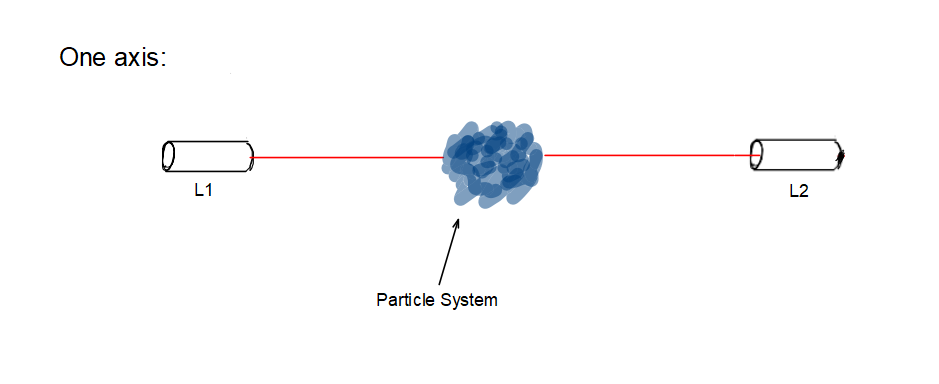
\includegraphics[scale = 0.4]{images/bimg.jpeg}
    \caption{}
\end{figure}

\noindent Suppose a particle in the system is stationary. The lasers have a non-resonant frequency, so the particle does not absorb the electromagnetic radiation of the lasers. Suppose now that the particle is moving toward laser 1 (L1 in the figure). According to the Doppler effect, the frequency of L2 is red shifted, moving its value further away from resonance; it is not absorbed. On the other hand, the frequency of L1 is blue-shifted, so it appears resonant. The particle absorbs the energy of the e.m. pulse, reverting it back to its original state/speed. A completely analogous thing happens for a particle moving toward L2. 

\subsubsection{A ``kind-of'' trapping: Optical molasses}
Having 6 lasers -or 3 lasers and mirrors respectively- forces the system of particles to a steady state, each axis operates as shown above. The particles become trapped in a specific cloud-like space (forced to perform random walks). The particles are not forced together by an external force (like a magnetic field) ; their directional motion is being constantly controlled by the lasers. For more information, see \href{https://en.wikipedia.org/wiki/Sisyphus_cooling}{polarization gradient cooling}.

\subsubsection{Doppler limit}
\tab The Doppler temperature limit refers to the minimum achievable temperature through Doppler cooling. When an atom absorbs a photon while moving in the opposite direction to the light source, its velocity decreases due to the conservation of momentum. Subsequently, when the excited atom spontaneously emits the absorbed photon, it receives a random momentum kick in a random direction. Since these spontaneous emissions occur in all directions equally, the average momentum kicks cancel out for the mean velocity. However, the mean squared velocity is non-zero, resulting in the supply of heat to the atom. At equilibrium, the rates of heating and cooling equalize, thereby creating a limit on the extent to which the atom can be cooled. Given that the transitions used in Doppler cooling have broad natural $\gamma$ rad/sec, this lower limit defines the lowest bound:

\begin{equation}
    T_{\text{Doppler}} = \frac{\hbar \cdot \gamma }{2\cdot k_{\beta} }
\end{equation}

\noindent
where $k_{\beta}$ is the Boltzmann constant and $\hbar$ is the reduced Planck constant, which is the lowest possible absolute temperature one can reach using Doppler cooling.

\subsection{Sideband Cooling}

\subsubsection{Cooling beyond the Doppler limit}
\tab Usually, the system on which sideband cooling is performed is a two-level system including a sufficiently cooled atom, or in our use case an ion. Modeling the system as a harmonic oscillator interacting with a classical electromagnetic field result s-after applying the rotating wave approximation- in the following familiar Hamiltonian:

\begin{equation}
    \hat{H} = \hat{H}_{H.O.} + \hat{H}_{al}
\end{equation}

\noindent with:

\begin{equation}
    \hat{H}_{H.O.} = \hbar v (n + \frac{1}{2})
\end{equation}

\begin{equation}
    \hat{H}_{al} = -\hbar\Delta\ket{e}\bra{e} + \hbar\frac{\Omega}{2}(\ket{e}\bra{g}\exp(ik\cdot r) + \ket{g}\bra{e}\exp(-ik\cdot r) )
\end{equation}

where:

$n$ is the number operator

$v$ is the frequency spacing of the oscillator

$\Omega$  is the \href{https://en.wikipedia.org/wiki/Rabi_frequency}{Rabi frequency} due to the atom-light interaction

$\Delta$  is the \href{https://en.wikipedia.org/wiki/Laser_detuning}{laser detuning} from $\omega_{0}$

$\mathbf{k}$  is the laser \href{https://en.wikipedia.org/wiki/Wave_vector}{wave vector}
\\
\\
\tab That is the Jaynes-Cummings Hamiltonian used to describe the phenomenon of an atom coupled to a cavity in quantum electrodynamics (skipping a lot of math for the sake of simplicity. For more, check Turchette et al.)



\end{document}